\begin{figure}[htp]
\centering

\begin{minipage}{.45\textwidth}
    \centering
    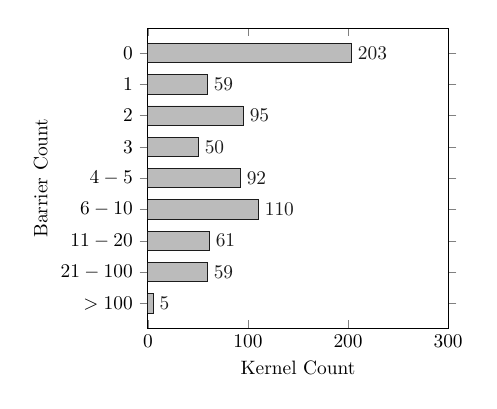
\begin{tikzpicture}[scale=0.7]
    
    \selectcolormodel{gray}
    
    \begin{axis}[
        xbar, xmin=0, xmax=300,
        xlabel={Kernel Count},
        symbolic y coords={
            {$> 100$},
            {$21-100$},
            {$11-20$},
            {$6-10$},
            {$4-5$},
            $3$,
            $2$,
            $1$,
            $0$
        },
        ytick=data,
        ylabel={Barrier Count},
        nodes near coords,
        nodes near coords align={horizontal},
        height=200pt, width=200pt
    ]
    
    \addplot coordinates {
        (5,{$> 100$})
        (59,{$21-100$})
        (61,{$11-20$})
        (110,{$6-10$})
        (92,{$4-5$})
        (50,$3$)
        (95,$2$)
        (59,$1$)
        (203,$0$)
    };
    
    \end{axis}
    \end{tikzpicture}
    
    \caption{Kernels with 'n' Instrumented Barriers}
    \label{Fi:kernels_barriers}
\end{minipage}

\end{figure}
